\newpage
\section{BPMN}

\subsection{Assumptions}
\begin{description}
\item[Website]\hfill \\
Endpoints are always possible. Therefor we leave out the modeling of it to not overload the models.
\item[Web-Application]\hfill \\ 
The Web-Application consist of the back-end as well as the front-end.
It is always listening for events, for that reason the Web-Application has a unconditional starting point.
\item[Web-Application non reachability]\hfill \\
We assume the system is allays reachable, for the point the system is not reachable we model in BPMN \textit{Content} for the login a work flow.
This could happen in a Web-Application at any point, therefore we do not consider it farther in the models. Also we usually not consider that the Actor can went through its history and can so revisited sites.
\item[Communication]\hfill \\ The communication between back-end and front-end uses a restful Api through sending JSON datas. 
\item[Roles]\hfill \\ 
The behavior of the Content-Manager is known, from the general Actor not.
The pool in the BPMN Model \textit{CRUD Content} of the Content-Manager is not a black box. The pool in the BPMN Model \textit{Search  CoffeeShop from Landingpage} of the Actor is a black box.
\end{description}


\newpage
\subsection{Content-Manager: CRUD Content}
The \textit{Content-Manager}(CM) is on the login page. The CM sends the \textit{Input-Form} for the login to the \textit{Web-Application}(WA). The System processes the data and eventually sends a response back.
Meanwhile the \textit{Content-Manager} waits for the response. The time for the WA might be to long and the CM gets a server error. This presents an endpoint.\\
Otherwise, if the CM gets a response back from the WA and it is a valid input the CM can proceed, or exclusively the response is  not valid and the CM can try to enter the input data again. The WA checks the input until it accept the login data.\\
The CM can now chooses which kind of content\{CoffeeShop, Article, Bean, Blend, BusStation, POI, Events \} he/she/it wants to processed by clicking on a corresponding tab. The WA gets the choice and renders the response for the CM.\\
The Content-Manager fills out the Input-Form of the tab and sends it to the WA. It might be a search request for a Content to edit or delete, as well as newly created content. The WA~(here the front-end) checks validate the input data. It gives a feedback and let the CM edit the input data to resend it if the input data is not valid. Otherwise, the WA response positive: this could be the Content to edit, or just that the input data is valid. The CM can keep editing and let the WA validate the new input, this process is presented in the \textit{finish?} loop. In the last cycle the CM sends the \textit{safe} command and the WA executes the corresponding data base operation. It sends back a response about the success status of the operation to  the CM.\\
The Content-Manager can chooses other Content to work on or end the Process. The log out process is not model here.


\begin{figure}[ht]
\includegraphics[
    page=1,
    width=\textwidth,
    height=\textheight,
    keepaspectratio
]{BPMN/content.png}
\vfill
\caption{BPMN: Content CRUD Process}
\end{figure}

\newpage
\subsection{Actor: Login}
The Web-Application is awaiting an \textit{Input-Form} from the \textit{Actor}. After receiving the input, it will check the data with the \textit{DataBase}. 
Based on the return result it wills reject or accept the \textit{Actor} input and sent the result back to the \textit{Actor}
\begin{figure}[th]
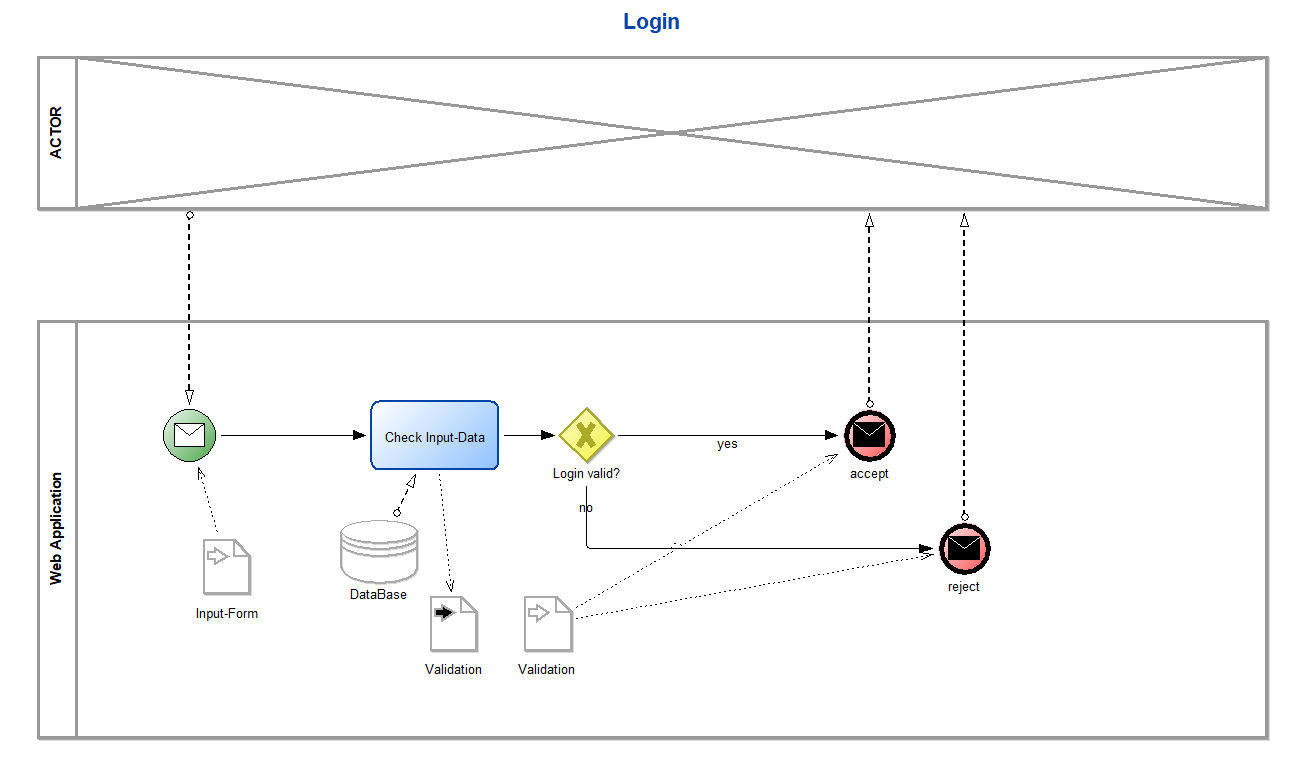
\includegraphics[
    page=1,
    width=\textwidth,
    height=\textheight,
    keepaspectratio
]{BPMN/Login.png}
\vfill
\caption{BPMN: Login Process}
\end{figure}


\newpage
\subsection{Actor: Search CoffeeShop from Landingpage}
The modeled search process starts at the Landingpage of the Website. The Web-Application(WA) waits for a search option. At this point it can be a request for \textit{Direct-Search}(Search for a CoffeeShop name) or a \textit{Quick-Search}(Search with reduced input parameters).\\
For the Direct-Search the input can be just some characters. The WA searches in the data base for all CoffeeShops which starts with the characters. It returns it as list to the Actor. The Actor can change the input and so let the WA search for the changed input. Alternative the Actor can request one of the CoffeeShops from the list. Than the WA gets the CoffeeShop from the data base and sends it to the Actor.\\
For the Quick-Search the Actor sends a \textit{Input-Form} with parameters. The WA queries the data base for it and returns a list of CoffeeShops, it also presents the Actor the \textit{Elaborate-Search} with all search parameters.\\
The Actor can now select a CoffeeShop from the list or add further search parameters. If the Actor change search parameters. The WA evaluate the search parameter and sent a list of matching CoffeeShops to the Actor.  If the Actor send a select request, the WA send the corresponding shop site back. From this point the Actor can begin a new search with pressing the back button or the \textit{Kaffee} button in the nav bar.

\begin{figure}[!th]
\includegraphics[
    page=1,
    width=\textwidth,
    height=\textheight,
    keepaspectratio
]{BPMN/search_landingpage.png}
\vfill
\caption{BPMN: Search Process from Landingpage}
\end{figure}

